 % --------------------------------------------------------------
% Based on a homework template by Dana Ernst (MTH320 Homework
% template on Overleaf).
% --------------------------------------------------------------

\documentclass[12pt]{article}

\usepackage{graphicx}
\graphicspath{{./images/}}
\usepackage[margin=1in]{geometry} 
\usepackage{amsmath,amsthm,amssymb}
% https://tex.stackexchange.com/questions/146306/how-to-make-horizontal-lists
\usepackage[inline]{enumitem} % allows using letters in enumerate list environment
\usepackage[mathscr]{euscript}
% source: https://stackoverflow.com/questions/3175105/inserting-code-in-this-latex-document-with-indentation

\usepackage{listings}
\usepackage{color}
\usepackage{hyperref}

\newtheorem{theorem}{Theorem}

\definecolor{dkgreen}{rgb}{0,0.6,0}
\definecolor{gray}{rgb}{0.5,0.5,0.5}
\definecolor{mauve}{rgb}{0.58,0,0.82}

\lstset{frame=tb,
	language=C, % language for code listing
	aboveskip=3mm,
	belowskip=3mm,
	showstringspaces=false,
	columns=flexible,
	basicstyle={\small\ttfamily},
	numbers=none,
	numberstyle=\tiny\color{gray},
	keywordstyle=\color{blue},
	commentstyle=\color{dkgreen},
	stringstyle=\color{mauve},
	breaklines=true,
	breakatwhitespace=true,
	tabsize=4
}

\newcommand{\N}{\mathbb{N}}
\newcommand{\Z}{\mathbb{Z}}

\newenvironment{ex}[2][Exercise]{\begin{trivlist}
		\item[\hskip \labelsep {\bfseries #1}\hskip \labelsep {\bfseries #2.}]}{\end{trivlist}}

\newenvironment{sol}[1][Solution]{\begin{trivlist}
		\item[\hskip \labelsep {\bfseries #1:}]}{\end{trivlist}}


\begin{document}

% --------------------------------------------------------------
%                         Start here
% --------------------------------------------------------------

\noindent Sergio Garcia Tapia \hfill

\noindent{\small Numerical Linear Algebra, Lloyd Trefethen and David Bau III} \hfill 

\noindent{\small Lecture 1: Matrix-Vector Multiplication} \hfill 

\noindent\today
\section*{Lecture 1: Matrix-Vector Multiplication}

\begin{ex}{1}
	Let $B$ be a $4\times 4$ matrix to which we apply the following operations:
	\begin{enumerate}
		\item double column 1,
		\item half row 3,
		\item add row 3 to row 1,
		\item interchange columns 1 and 4,
		\item subtract row 2 from each of the other rows,
		\item replace column 4 by column 3,
		\item delete column 1 (so that the column dimension is reduced by 1).
	\end{enumerate}
	\begin{enumerate}[label=(\alph*)]
		\item Write the result as a product of eight matrices.
		\item Write it again as a product $ABC$ (same $B$) of three matrices.
	\end{enumerate}
\end{ex}

\begin{sol}
	\
	\begin{enumerate}[label=(\alph*)]
		\item To perform any operation on the columns, we can multiply by a matrix on the right,
		thinking of its columns as the weights that will be used to create a linear combination
		of the columns of the operand matrix. For example, to double column 1 of $B$, we multiply
		$B$ on the right by $D_1$, where
		\begin{align*}
			D_1=\begin{bmatrix}
				2 & 0 & 0 & 0\\
				0 & 1 & 0 & 0\\
				0 & 0 & 1 & 0\\
				0 & 0 & 0 & 1
			\end{bmatrix}
		\end{align*}
		We now have $BD_1$. To perform row operations, we can instead operate with the transpose
		by relying on the identity
		\[
			(SR)^T=R^TS^T
		\]
		This enables us to think of the row operations as column operations. For example, to
		halve row 3 of $BD_1$, we instead think of halving column 3 of its transpose $(BD_1)^T$.
		Doing this is simply multiplying by $D_2^T$ on the right, where
		\begin{align*}
			D_2^T=\begin{bmatrix}
				1 & 0 & 0 & 0\\
				0 & 1 & 0 & 0\\
				0 & 0 & \frac{1}{2} & 0\\
				0 & 0 & 0 & 1
			\end{bmatrix}
			D_2=\begin{bmatrix}
				1 & 0 & 0 & 0\\
				0 & 1 & 0 & 0\\
				0 & 0 & \frac{1}{2} & 0\\
				0 & 0 & 0 & 1
			\end{bmatrix}
		\end{align*}
		Now we have $(BD_1)^TD_2^T$, which is equivalent to $D_2(BD_1)$. To add row 3 to row 1,
		we perform the equivalent of adding column 3 to column 1 of the transpose. To achieve this,
		we multiply the transpose on the right of our result so far by
		$D_3^T$, where
		\begin{align*}
			D_3^T = \begin{bmatrix}
				1 & 0 & 0 & 0\\
				0 & 1 & 0 & 0\\
				3 & 0 & 1 & 0\\
				0 & 0 & 0 & 1
			\end{bmatrix}
			\quad \quad
			D_3 = \begin{bmatrix}
				1 & 0 & 3 & 0\\
				0 & 1 & 0 & 0\\
				0 & 0 & 1 & 0\\
				0 & 0 & 0 & 1
			\end{bmatrix}
		\end{align*}
		Operating on the transpose results in $(D_2BD_1)^TD_3^T$, which is equivalent to the
		product $D_3D_2BD_1$. Next, to interchange columns 1 and 4, we multiply on the right by
		\begin{align*}
			D_4 = \begin{bmatrix}
				0 & 0 & 0 & 1\\
				0 & 1 & 0 & 0\\
				0 & 0 & 1 & 0\\
				1 & 0 & 0 & 0
			\end{bmatrix}
		\end{align*}
		Thus we have $(D_3D_2BD_1)D_4$. To subtract row 2 from each of the other rows,
		we again think of it in terms of columns by using the transpose. This translates to
		subtracting column 2 of the transpose from the other transposed columns. To achieve
		this, we multiply the transpose of our result so far on the right by $D_5^T$, where
		\begin{align*}
			D_5^T=\begin{bmatrix}
				 1 & 0 &  0 &  0\\
				-2 & 1 & -2 & -2\\
				 0 & 0 &  1 &  0\\
				 0 & 0 &  & &  1
			\end{bmatrix}
			\quad \quad
				D_5=\begin{bmatrix}
				1 & -2 & 0 & 0\\
				0 &  1 & 0 & 0\\
				0 & -2 & 1 & 0\\
				0 & -2 & 0 & 1
			\end{bmatrix}
		\end{align*}
		This gives $(D_3D_2BD_1D_4)^TD_5^T$, so using our identity gives $D_5(D_3D_2BD_1D_4)$.
		To replace column 4 by column 3, we multiply by $D_6$ on the right:
		\begin{align*}
			D_6=\begin{bmatrix}
				1 & 0 & 0 & 0\\
				0 & 1 & 0 & 0\\
				0 & 0 & 1 & 1\\
				0 & 0 & 0 & 0
			\end{bmatrix}
		\end{align*}
		Now our product is $(D_5D_3D_2BD_1D_4)D_6$. Finally, to delete column 1, we multiply
		on the right by $D_7$, where
		\begin{align*}
			D_7=\begin{bmatrix}
				0 & 0 & 0 & 0\\
				0 & 1 & 0 & 0\\
				0 & 0 & 1 & 0\\
				0 & 0 & 0 & 1
			\end{bmatrix}
		\end{align*}
		Our final result is $(D_5D_3D_2BD_1D_4D_6)D_7$, which is a product of 8 matrices.
		\item We let $A=D_5D_3D_2$ and $C=D_1D_4D_7$.
	\end{enumerate}
\end{sol}

\begin{ex}{2}
	Suppose masses $m_1,m_2,m_3,m_4$ are located at positions $x_1$, $x_2$, $x_3$, $x_4$ in a line and
	connected by springs with constants $k_{12}$, $k_{23}$, $k_{34}$ whose natural lengths of extension
	are $\ell_{12}$, $\ell_{23}$, $\ell_{34}$. Let $f_1$, $f_2$, $f_3$, $f_4$ denote the rightward forces
	on the masses, e.g., $f_1=k_{12}(x_2-x_1-\ell_{12})$.
	\begin{enumerate}[label=(\alph*)]
		\item Write a $4\times 4$ matrix equation relating the column vectors $f$ and $x$. Let
		$K$ denote the matrix in this equation.
		\item What are the dimensions of the entries of $K$ in the physics sense (e.g., mass times
		time, distance divided by mass, etc.)?
		\item What are the dimensions of $\det(K)$, again in the physics sense?
		\item Suppose $K$ is given numerical values based on the units meters, kilograms, and
		seconds. Now the system is rewritten with a matrix $K'$ based on centimeters, grams,
		and seconds. What is the relationship of $K'$ to $K$? What is the relationship of
		$\det(K')$ to $\det(K)$?
	\end{enumerate}
\end{ex}

\begin{sol}
	\
	\begin{enumerate}[label=(\alph*)]
		\item 	See Figure~\ref{ex:1.2} for a picture I have created of the scenario described.
		\begin{figure}
			\centering
			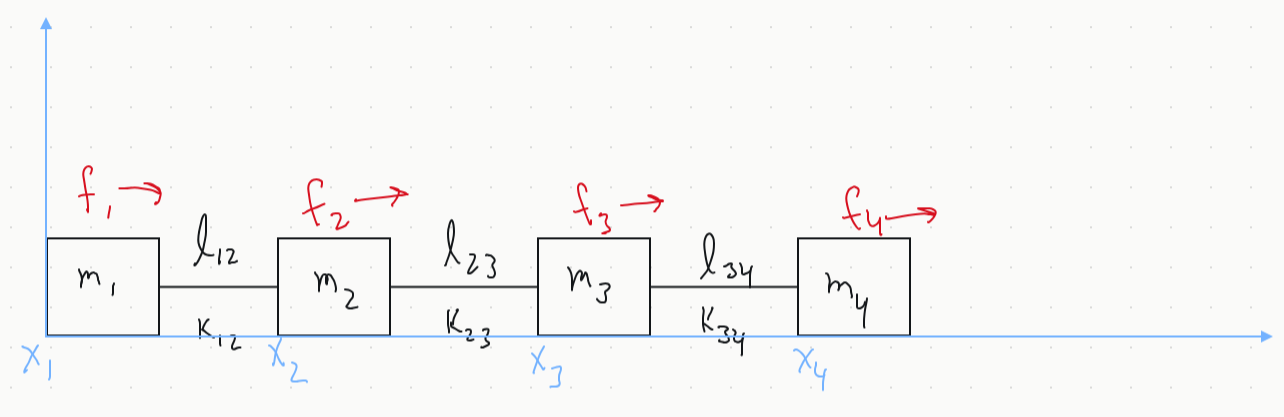
\includegraphics[width=0.7\textwidth]{exercise-01-02-hookes-law}
			\caption{Exercise 1.2: Block masses connected by springs in a line}
			\label{ex:1.2}
		\end{figure}
		I presume that the force $f_1$ is calculated according to \emph{Hooke's Law}, giving
		rightward force on $m_1$ as the product of the spring constant $k_{12}$ connecting
		$m_1$ and $m_2$ and the displacement of that spring from its relaxed position.
		When $x_2-x_1=\ell_{12}$, the spring is relaxed, and hence there is no force. When
		mass $m_2$ is pulled right so that $x_2-x_1>\ell_{12}$, the displacement $x_2-x_1-\ell_{12}$
		is positive, inducing a force $f_1$ on $m_1$ that pulls $m_1$ rightward, and similarly,
		a leftward force $-f_1$ on $m_2$ pulling $m_2$ leftward. Since we are only asked
		for the rightward forces, and not the net force on each mass, we have
		\begin{align*}
			f_1&=k_{12}(x_2-x_1-\ell_{12})\\
			f_2&=k_{23}(x_3-x_2-\ell_{23})\\
			f_3&=k_{34}(x_4-x_3-\ell_{34})\\
			f_4&=0
		\end{align*}
		We can compactly summarize this with the matrix equation $f=K(x-l)$, where
		\begin{align*}
			f=\begin{bmatrix}
				f_1\\
				f_2\\
				f_3\\
				f_4
			\end{bmatrix}
			\quad
			x=\begin{bmatrix}
				x_1\\
				x_2\\
				x_3\\
				x_4
			\end{bmatrix}
			\quad
			\ell=\begin{bmatrix}
				0\\
				\ell_{12}\\
				\ell_{23} + \ell_{12}\\
				\ell_{34} + \ell_{23} + \ell_{12}\\
			\end{bmatrix}
			\quad
			K=\begin{bmatrix}
				-k_{12} & k_{12} & 0 & 0\\
				0 & -k_{23} & k_{23} & 0\\
				0 & 0 & -k_{34} & k_{34}\\
				0 & 0 & 0 & 0
			\end{bmatrix}
		\end{align*}
		\item $f_i$ has force dimensions and $x$ and $\ell$ have length dimensions.
		Thus each entry of $k$ results from their ratio, which in turn has
		dimensions of force divided by length.
		\item The dimensions of $\det(K)$ are force divided by length, all raised to
		the fourth power.
		\item If $K$ is given in units of meters, kilograms, and seconds, then the
		dimensions of the entry of $K$ are given in the units $\frac{kg\cdot m}{s^2}$,
		where $kg$ stands for kilograms, $m$ for meters, and $s$ for seconds.
		Meanwhile, $K'$ is given in dimensions centimeters, grams, and seconds, which
		is $\frac{g\cdot cm}{s^2}$. Since $1kg=1000g$, and $1m=100cm$, we see that
		$\frac{kg\cdot m}{s^2}=\frac{1000g\cdot 100cm}{s^2}=10^6\frac{g\cdot cm}{s^2}$.
		Thus, the relationship between $K$ and $K'$ is $K'=10^6\cdot K$. Since
		$\det(AB)=\det(A)\det(B)$, it follows that$\det(K')=\det(10^6I\cdot K)=10^6\cdot\det(K)$,
		where $I$ is the identity matrix.
	\end{enumerate}
\end{sol}

\begin{ex}{3}
	Generalizing Example 1.3, we say that a square or rectangular matrix $R$ with entries
	$r_{ij}$ is \emph{upper-triangular} if $r_{ij}=0$ for $i>j$. By considering what space
	is spanned by the first $n$ columns of $R$ using (1.8), show that if $R$ is a nonsingular
	$m\times m$ upper-triangular matrix, the $R^{-1}$ is also upper-triangular.
	(The analogous result also holds for lower-triangular matrices).
\end{ex}

\begin{sol}
	\
	\begin{proof}
		If $R$ is nonsingular, then it has a unique inverse $R^{-1}$ such that
		\[
		I=R^{-1}R=RR^{-1}
		\]
		where $I$ is the $m\times m$ identity matrix. Denote the $j$-th column of $I$
		by $e_j$ for $j\in\{1,\ldots,m\}$, and the $i$-th column of $R^{-1}$ by $z_i$.
		Then since $I=R^{-1}R$, the $j$-th column of $I$ is a linear combination of the columns
		of $R^{-1}$ using the entries in the $j$-th column of $R$. By (1.8), we have
		\begin{align*}
			e_j&=\sum_{i=1}^{m}r_{ij}z_i=\sum_{i=1}^{j}r_{ij}z_i
		\end{align*}
		To show that $z_{ij}=0$ for $i>j$, we proceed by induction on $j$, the column
		index. If $j=1$,
		then
		\begin{align*}
			e_1 = \sum_{i=1}^{1}r_{i1}z_i=r_{11}\cdot z_1
		\end{align*}
		The first entry in $e_1$ is 1 and the rest are 0. Since $R$ is nonsigular
		and upper-triangular, its diagonal entries are nonzero, so $a_{11\neq 0}$.
		Dividing by $a_{11}$ shows that $z_1=\frac{1}{a_{11}}e_1$, and hence,
		$z_{i1}=0$ for $i>1$.
		
		\
		Suppose $j>1$ and the result holds for all columns of smaller column indices
		Now
		\begin{align*}
			e_j&=\sum_{i=1}^{j}r_{ij}z_i=r_{jj}z_j + \sum_{i=1}^{j-1}r_{ij}z_i\\
			z_j&=\frac{1}{r_{jj}}e_j+\frac{1}{r_{jj}}\sum_{i=1}^{j-1}r_{ij}z_i
		\end{align*}
		Note that $r_{jj}\neq 0$ because $R$ is a nonsingular upper-triangular matrix.
		By our inductive hypothesis, $z_{ik}=0$ for $i>k$ whenever $1\leq i\leq j-1$.
		Since the scalar multiple $\frac{1}{r_{jj}}e_j$ of $e_j$ only has a nonzero
		entry in its $j$-th slot, it satisfies $e_{ij}=0$ for $i>j$. Since $z_{ij}$
		is their sum as seen above, we conclude that it too satisfies $z_{ij}=0$
		for $i>j$. We conclude by induction that $R^{-1}$ is upper-triangular.
	\end{proof}
\end{sol}

\begin{ex}{4}
	Let $f_1,\ldots,f_8$ be a set of functions ont he interval $[1,8]$, with the property
	that for any numbers $d_1,\ldots,d_8$, there exists a set of coefficients $c_1,\ldots,c_8$
	such that
	\[
	\sum_{j=1}^{8}c_jf_j(i)=d_i,\quad i=1,\ldots,8
	\]
	\begin{enumerate}[label=(\alph*)]
		\item Show by appealing to the theorems of this lecture that $d_1,\ldots,d_8$ determine
		$c_1,\ldots,c_8$ uniquely.
		\item Let $A$ be the $8\times 8$ matrix representing the linear mapping from data
		$d_1,\ldots,d_8$ to coefficients $c_1,\ldots,c_8$. What is the $i,j$ entry of $A^{-1}$?
	\end{enumerate}
\end{ex}

\begin{sol}
	\
	\begin{enumerate}[label=(\alph*)]
		\item \begin{proof}
			Let $F$ be the $8\times 8$ matrix whose $j$-th column $f_j$ represents the
			column vector $(f_j(1),\ldots,f_j(8))$, where $j\in\{1,\ldots,8\}$. The
			given information implies that $\text{rank}(F)=~8$. By Theorem 1.3, this
			implies that $\text{null }(A)=\{0\}$. Thus, $d_1,\ldots,d_8$ determines
			$c_1,\ldots,c_8$ uniquely. Otherwise, if there is another list of
			coefficients $c_1',\ldots,c_8'$ that also yield $d_1,\ldots,d_8$, then
			the list $c_1-c_1',\ldots,c_8-c_8'$ yields $d_1-d_1,\ldots,d_8-d_8$;
			that is, it yields the 0 vector. Since $\text{null }(A)=\{0\}$, this
			implies that $c_i=c_i'$ for all $i\in\{1,\ldots,8\}$, and hence the
			$c_i$'s are uniquely determined.
		\end{proof}
		\item Per the description of $A$ and our definition of $F$, we see that $A=F^{-1}$,
		and hence $A^{-1}=F$. Thus, the $i,j$ entry of $A^{-1}$ is the value of the
		$j$-th function at $i$.
	\end{enumerate}
\end{sol}

\end{document}